\chapter{Method}\label{ch:method}

The Hückel and Hartree-Fock approximations were both implemented in Python using the NumPy, SciPy, and Matplotlib libraries. These methods were separated into general functions, that were used to generate atomic positions and basis functions, and specific functions used to generate and solve the Hamiltonian matrices for each method. Atomic units were used in these scripts to simplify calculations. Refer to Table \ref{tab:measuredconstants} below for the atomic-unit constants and conversion factors used \cite{noauthor_appendix_2012}.

\vspace{0.5cm}
\begin{table}[h!]
\begin{center}
\begin{tabular}{ l l l c l}\hline
\textbf{Description}  & \textbf{} & \textbf{Value (Atomic)} & \textbf{} & \textbf{Value (SI)}\\ \hline
Electronic charge & $e$ & 1 & or & $1.60218 \cdot 10^{-19} \; \coulomb$ \\
Proton mass            & $m_{p}$ & $1.83615 \cdot 10^{3}$ & or &  $1.67262 \cdot 10^{-27} \; \kilo\gram$ \\
Neutron mass            & $m_{n}$ & $1.83835 \cdot 10^{3}$ & or &  $1.67493 \cdot 10^{-27} \; \kilo\gram$ \\
Electron mass          & $m_{e}$ & 1 & or &  $9.10938 \cdot 10^{-31} \; \kilo\gram$ \\
Permittivity of vacuum & $\epsilon_{0}$ & $1/4\pi$ & or &  $8.85419 \cdot 10^{-12} \; \farad\per\meter $ \\
Speed of light in vacuum & $c$               & $1.37036 \cdot 10^2$ & or &  $2.99792 \cdot 10^{8} \; \meter\per\second $ \\ 
Planck constant        & $h$ & $2\pi$ & or &  $6.62607 \cdot 10^{-34} \; \joule\cdot\second$ \\
Reduced Planck constant        & $\hbar$ & 1 & or &  $1.0546 \cdot 10^{-34} \; \joule\cdot\second$ \\
Electron volt        & $eV$ & $3.67493 \cdot 10^{-2}$ & or &  $1.60218 \cdot 10^{-34} \; \joule$ \\
Bohr radius        & $a_0$ & 1 & or &  $5.29177 \cdot 10^{-11} \; \meter$ \\
Angstrom        & $\mathring{A}$ & $1.88973$ $a_0$ & or &  $1 \cdot 10^{-10} \; \meter$ \\
\hline
\end{tabular}
\end{center}
\caption{A table of the relevant constants and conversion factors used in this experiment, in both atomic and SI units. The results in this report were calculated using atomic units, which both simplified manual calculations and accelerated project code execution.}
\label{tab:measuredconstants}
\end{table}


\section{Molecule Construction}\label{sec:moleculeconstruction}

The atomic positions corresponding to Benzene and Graphene molecules were both calculated in different ways within the project script. For Benzene, molecules were created by first choosing a central point, and then distributing atoms around this point at equal radii but evenly spaced azimuthal angles. For the Hückel method, only Carbon atoms were distributed in this way, but for the Hartree-Fock approximation, both Carbon and Hydrogen atoms were distributed at equal angles but different radii. Here, the radii chosen were $R_C = R_{(CC)} = 1.3913$ $\mathring{A}$, and $R_H = R_{(CC)} + R_{(CH)} = 2.4722$ $\mathring{A}$, corresponding to existing experimental values \cite{esselman_precise_2023}. Refer to Figure \ref{fig:benzenestructure} below for the resulting atomic positions used for Benzene.\\\\\\\\

\begin{figure}[h!]
\begin{center}
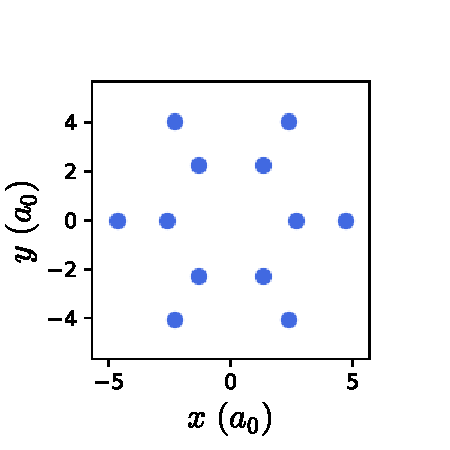
\includegraphics[width=0.4\linewidth]{figures/BenzeneStructure.pdf}
\end{center}
\caption{Molecular structure of the Benzene molecule considered in this report. The Carbon atoms are separated by 1.3913 angstrom, or approximately 2.63 Bohr radii ($a_0$). The Hydrogen atoms are then 1.0809 angstrom, or approximately 2.04 Bohr radii ($a_0$) from the nearest Carbon atom.}
\label{fig:benzenestructure}
\end{figure}


For the hexagonal lattice of Graphene, a more complex method was used. The Carbon atoms were first arranged in rows, and were then offset horizontally to create a triangular lattice. After this, the script iterated through lattice positions, and removed atoms that lay at hexagonal centre-points, creating the desired hexagonal lattice. Here, the lattice points were spaced at distances of $R_{CC} = 1.42$ $\mathring{A}$, corresponding to their experimental separation \cite{yang_structure_2018}. Refer to Figure \ref{fig:graphenestructures} below for the three Graphene lattices used in this report, $G_1$, $G_2$, and $G_3$, which were created using initial row sizes of 5, 7, and 10 atoms respectively.\\\\


\begin{figure}[h!]
\begin{center}
\hspace*{-1.6cm}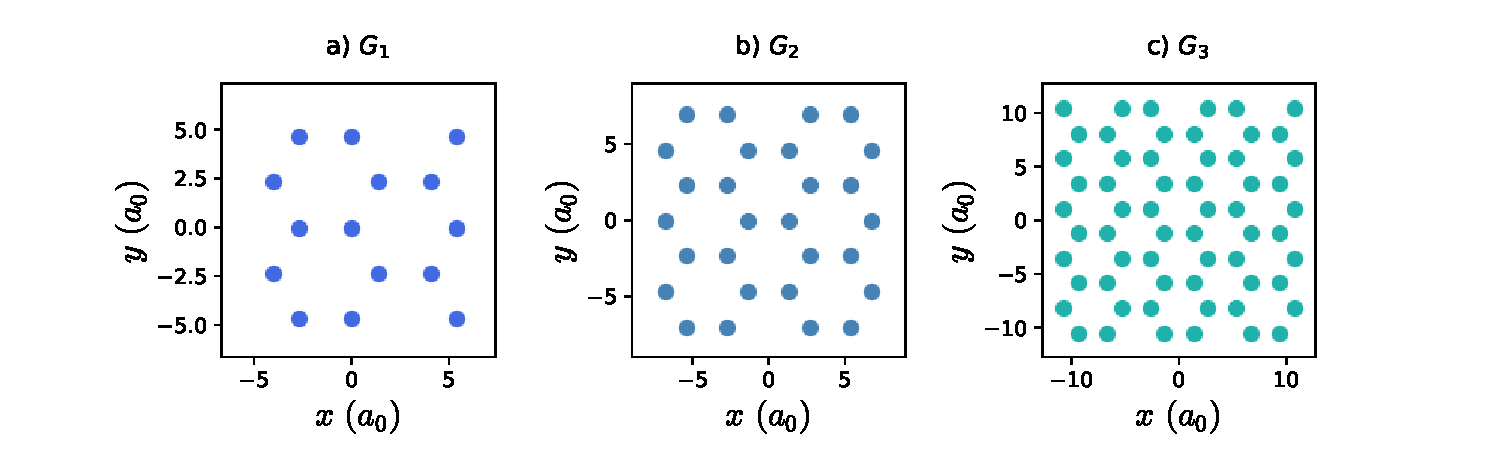
\includegraphics[width=1.2\linewidth]{figures/GrapheneStructures.pdf}
\end{center}
\caption{Crystal structures of the three Graphene flakes considered in this report. The $G_1$, $G_2$ and $G_3$ crystal lattices have totals of 15, 28 and 60 Carbon atoms, respectively. The neighbouring atoms in each lattice are separated by 1.42 angstrom, or approximately 2.68 Bohr radii ($a_0$).}
\label{fig:graphenestructures}
\end{figure}


\section{Hückel Approximation}\label{sec:huckelmethod}

Slater basis functions (\ref{eq:Slater}) corresponding to the quantum numbers $l=1$ and $m=0$, and parameter $\lambda=1.2$, were calculated for both Benzene and Graphene, over spatial domains of 10 and 20 Bohr radii respectively, and with 3D resolutions of (50x50x50) cells. With these, Hückel method Hamiltonians (\ref{eq:HuckelMatrix}) for each system were also found, following their cyclic-planar structures. The following interaction matrix was used for Benzene, with the positions of the $\alpha$ and $\beta$ parameters corresponding to a ring of Carbon atoms, each with two atomic neighbours:

\vspace{0.2cm}
\begin{equation}\label{eq:HuckelBenzeneMatrix}
\vect{F^{(Benzene)}} = 
  \left(\begin{array}{c c c c c c}
    \alpha & \beta & 0 & 0 & 0 & \beta \\
    \beta & \alpha & \beta & 0 & 0 & 0 \\
    0 & \beta & \alpha & \beta & 0 & 0 \\
    0 & 0 & \beta & \alpha & \beta & 0 \\
    0 & 0 & 0 & \beta & \alpha & \beta \\
    \beta & 0 & 0 & 0 & \beta & \alpha \\
  \end{array}\right)
\end{equation}
\vspace{0.2cm}

The interaction matrices for each Graphene crystal were constructed algorithmically by finding the nearest 2-3 neighbours to each Carbon atom, and placing $\beta$ values at their associated matrix indices. For both Benzene and Graphene, the parameter values $\alpha = -0.6$ and $\beta = -0.1$ were used, corresponding to the $2p_z$ orbital energy and average interaction energy of Carbon atoms, respectively \cite{quiney_art_nodate}. From these $\boldsymbol{F}$ and $\boldsymbol{S}$ interaction matrices, the general eigenvalue equations were then solved numerically, producing electron orbital eigenvalues and wavefunctions for each system. These were plotted, and then compared with known results \cite{neto_electronic_2009}.

\section{Hartree-Fock Approximation}\label{sec:hartreemethod}

Gaussian basis functions (\ref{eq:Gaussian}) were first calculated for a range of Hydrogen systems, using the geometric basis set with $\alpha=0.001$ and $\beta=1.9$, and over spatial domains ranging from 10 to 40 Bohr radii. Basis functions for the orbital quantum numbers $l=0$, $l=1$ and $l=2$ were generated with domain resolutions of (50x50x50), and the atomic Hartree-Fock $\boldsymbol{S}$, $\boldsymbol{T}$ and $\boldsymbol{V}$ matrices (\ref{eq:AtomicS} - \ref{eq:AtomicV}) were each calculated, combined, and solved numerically for the lowest-energy $s$, $p$ and $d$ states of Hydrogen. The resulting eigenvalues and wavefunctions were then plotted, and compared with expected results \cite{walczak_hydrogen_2013}.\\

In further comparison, these steps were repeated using both the molecular Hartree-Fock equations (\ref{eq:MolecularS} - \ref{eq:MolecularV}), and a fully-numerical implementation of the Hartree-Fock matrix integrals (\ref{eq:HartreeFockS} - \ref{eq:HartreeFockG}), without the simplified analytic forms from (\ref{eq:AtomicS}) onwards. These resulting wavefunctions and eigenvalues were plotted and compared with the existing analytic, atomic results for $s$-shell, $l=0$, $m=0$ Hydrogen, to verify the accuracy of each method. Additionally, the calculation times for the analytic and numerical $s$-shell Hydrogen orbitals were also measured and compared, to determine the relative practicality of the numerical method.\\

Finally, additional Gaussian basis functions and molecular Hartree-Fock matrices were calculated for the atomic and molecular structures of Helium, Benzene and $G_2$ Graphene, over spatial domains from 10 to 40 Bohr radii. The resulting wavefunctions for Helium were calculated both with and without the addition of the atomic Hartree-Fock potential $G^{(HF)}$ (\ref{eq:HartreeFockG}), and these results were compared with known values \cite{nascimento_determination_2005} to evaluate the accuracy of both algorithms used. The eigenvalues and wavefunctions calculated for Benzene and Graphene were then both compared with their associated Hückel theory results.